\documentclass{standalone}
\usepackage{tikz}
\usepackage{ctex,siunitx,ninecolors}
\setCJKmainfont{Noto Serif CJK SC}
\usepackage{tkz-euclide}
\usepackage{amsmath}
\usepackage{wasysym}
\usetikzlibrary{patterns, calc}
\usetikzlibrary {decorations.pathmorphing, decorations.pathreplacing, decorations.shapes,}
\begin{document}
\small
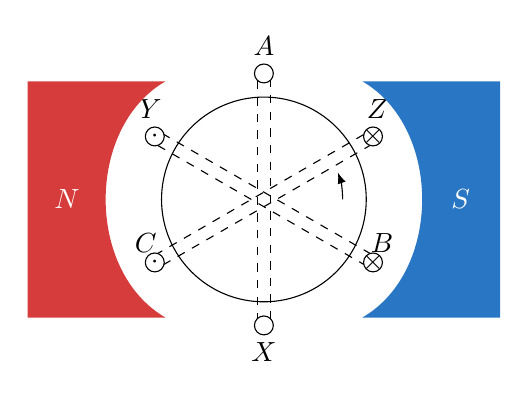
\begin{tikzpicture}[>=latex,scale=1]
  % \useasboundingbox(0.9,0)rectangle(5.1,5);
  \draw (0,0) circle (1.3);
  \foreach \x in {30,90,150}
  {
      \draw [rotate=\x, dashed] (-1.6,-.08) rectangle (1.6,.08);
  }
      \foreach \x in {30,90,150}
  {        
      \draw (\x:1.6) [fill=white] circle (0.12);
      \draw (-\x:1.6) [fill=white] circle (0.12);
  }
  \node at (30:1.6){$\times$};
  \node at (-30:1.6){$\times$};
  \node at (150:1.6){$\cdot$};
  \node at (-150:1.6){$\cdot$};
  \draw [->] (1,0) arc (0:20:1);
  \node at (32:1.7)[above]{$Z$};
  \node at (-28:1.7)[above]{$B$};
  \node at (150-2:1.7)[above]{$Y$};
  \node at (-150-2:1.7)[above]{$C$};
  \node at (90:1.7)[above]{$A$};
  \node at (-90:1.7)[below]{$X$};
  \fill[azure5] (1.25,1.5) to [bend left=60](1.25,-1.5)--(3,-1.5)--(3,1.5)--cycle;
  \fill[red5] (-1.25,1.5) to [bend left=-60](-1.25,-1.5)--(-3,-1.5)--(-3,1.5)--cycle;
  \node at (-2.5,0)[text=white]{$N$};\node at (2.5,0)[text=white]{$S$};
\end{tikzpicture}
\end{document}